\chapter{Trabalhos Relacionados}\label{cap:trabrel}
%==================================================================
% - Breve explicação
% - Contribuição do artigo
% - Funcionamento básico de método (como chegou na contribuição)
% - Dados usados
% - Tratamento dos dados
% - Features
% - Construção das features
% - Sobre os modelos
% - Conclusão
%==================================================================

% introdução
Neste capítulo serão descritos os principais trabalhos relacionados a este projeto de conclusão de curso.
O capítulo será dividido em duas seções: a primeira delas constituída por alguns trabalhos que identificam discurso de ódio através de modelos de predição, alguns métodos para a criação de novos atributos que ajudam na predição dos dados, bem como os resultados de seus modelos (Seção \ref{sec:trabrel-1}). Na segunda seção é realizada uma análise sobre a extração de meta-atributos (atributos que possuem relação com os atributos originais), utilizando \textit{KNN} para obter informações relevantes de documentos similares, bem como uma análise sobre os seus resultados (Seção \ref{sec:trabrel-2}).

\section{Identificação de discurso de ódio}\label{sec:trabrel-1}

\subsection{Detecção automatizada de discurso de ódio e o problema da linguagem ofensiva}\label{sec:trabrel-1.1}

% objetivo do trabalho
O trabalho de \cite{davidson2017automated} tem por objetivo a classificação em três classes de textos (documentos): discurso de ódio, discurso ofensivo e não ofensivo. O discurso de ódio é definido, conforme \cite{nockleby2000hate}, como qualquer comunicação que deprecie uma pessoa ou um grupo com base em alguma característica como raça, cor, etnia, gênero, orientação sexual, nacionalidade, religião ou outras. Já discurso ofensivo é categorizado, segundo \cite{davidson2017automated}, como documentos que têm linguagem ofensiva mas que não discrimina as pessoas ou um grupo de pessoas.

O discurso de ódio pode ser usado de diferentes maneiras: 
\begin{itemize}
    \item Pode ser enviado diretamente para uma pessoa ou grupo de pessoas;
    \item Pode ser direcionado para ninguém em particular (sarcasmo, ironia);
    \item Em conversas entre pessoas (comentários de redes sociais, fóruns de discussão, sala de bate-papos, etc).
\end{itemize}

%Em muitos trabalhos que tentam classificar um determinado documento como discurso de ódio ou não, 
Neste trabalho é proposta a divisão entre discurso de ódio e discurso ofensivo por alguns motivos. Em muitos casos, textos apresentam palavras ofensivas, mas que de fato não expressam ódio contra outras pessoas, por exemplo, o uso do sarcasmo entre amigos, muitas vezes considerado como brincadeira. Esse tipo de linguagem é comum nas mídias sociais \cite{kwok2013locate}, tornando a tarefa de classificação crucial para qualquer sistema que tente detectar discurso de ódio em documentos.

% como gerou a base
Para a construção dos dados foram utilizadas palavras e frases (\textit{tokens}) de ódio retiradas de um repositório \textit{on-line}\footnote{\url{https://www.hatebase.org/}} de discurso de ódio. Com esse conjunto de palavras e frases, foi feita uma seleção de \textit{tweets} que continham esses \textit{tokens}, resultando em 33.458 de usuários do twitter e 85,4 milhões de documentos (todos em inglês). Desses dados foram selecionados aleatoriamente 25.000 documentos para realização do experimento.

A classificação desses documentos foi realizada por pessoas (garantindo uma classificação mais correta) que tinham que escolher/votar em uma das três categorias que o documento pertencesse: discurso de ódio, discurso ofensivo e não ofensivo. Os classificadores foram instruídos que a presença de uma determinada palavra, embora ofensiva, não indica necessariamente que um documento é discurso de ódio. Cada documento foi classificado três ou mais vezes, sendo enquadrado na categoria que obteve mais votos. Depois dessa classificação manual, resultaram 24.802 documentos rotulados, alguns desconsiderados pela falta de votos.

Apenas 5\% dos documentos foram rotulados como discurso de ódio pela maioria dos classificadores e apenas 1,3\% foram classificados de forma unânime. A maioria dos documentos foi considerada discurso ofensivo (76\% classificados com 2/3 votos, 53\% classificados com 3/3 votos) e o restante foi considerado não ofensivo (16,6\% classificado de 2/3, 11,8\% em 3/3 vezes).

% construção dos atributos
Para a construção dos atributos, cada documento foi formatado em letras minúsculas para evitar divergências. Também foi utilizado o algoritmo de{\it Porter stemmer} para a remoção dos sufixos das palavras e o {\it N-gram} para a construção dos atributos, com os valores de $N={1,2,3}$. A atribuição dos pesos para os atributos foi feita {\it TF-IDF}. (veja na Seção \ref{sec:tfidf}.). Para capturar informações sintáticas dos textos foi usado {\it Part-of-Speech (POS)} juntamente com {\it N-gram} para gerar novos atributos que caracterizam informações da estrutura sintática dos documentos. Para capturar a qualidade de cada documento foi usado o cálculo de {\it Flesch Reading Ease}, que indica se o texto é compreensível para a leitura, onde os valores vão de 0 a 100; quanto maior a pontuação, mais fácil é a leitura. 

Outras características aplicadas no trabalho, levando em consideração os documentos utilizados, foram valores quantitativos extraídos dos textos como a contagem de \textit{hashtags}, menções, \textit{retweets} e \textit{URLs}, bem como recursos para o número de caracteres, palavras e sílabas em cada \textit{tweet}.

% construção do modelo
Para criação do modelo de predição foram testados uma variedade de modelos: regressão Logística, \textit{Naive Bayes}, Árvores de Decisão, Florestas Aleatórias e o \textit{SVM}. Cada modelo foi testado usando validação cruzada de 5 vezes, mantendo 10\% da amostra para avaliação. Os resultados do \cite{davidson2017automated} mostram que Regressão Logística e \textit{SVM} tendem a ter um desempenho significativamente melhor do que outros modelos.

\begin{figure}[ht]
  \centering
  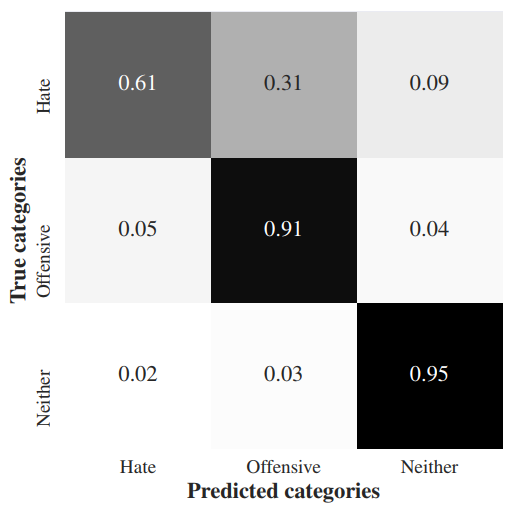
\includegraphics[height=0.4\textheight]{figuras/trab1-confusion-matriz.png}
  \caption{Matriz de confusão dos resultados com \textit{F1-Score} \cite{davidson2017automated}.}
  \label{fig:tb1confmatriz}
\end{figure}

Segundo o artigo, o classificador com melhor desempenho teve uma precisão geral de 91\%, revocação de 90\% e pontuação de F1 de 90\%. No entanto, observando a Figura \ref{fig:tb1confmatriz} percebe-se que quase 40\% dos discursos de ódio são classificados incorretamente: os resultados de precisão e revocação para a classe de ódio são 44\% e 61\%, respectivamente. A maior parte da classificação incorreta ocorre no triângulo superior da matriz, sugerindo que o modelo é favorável a classificar os documentos como menos ódio ou ofensivos do que os codificadores humanos. Um menor número de documentos são classificados como mais ofensivos ou odiosos do que sua verdadeira categoria, aproximadamente 5\% de documentos ofensivos e 2\% de não-ofensivo foram erroneamente classificados como discurso de ódio. 

\subsection{Detecção de Linguagem Abusiva em Conteúdos Online}\label{sec:trabrel-1.2}

% objetivo do trabalho
Em \cite{nobata2016abusive} são utilizados vários métodos de Processamento de Linguagem Natural (PLN) para criação de atributos. Tal trabalho combina algumas características do trabalho apresentado na Seção \ref{sec:trabrel-1.1} e propõe alguns novos atributos para  aprimorar os  resultados. Diversos métodos de PLN foram usados em trabalhos anteriores até então estudados, mas esses recursos nunca foram combinados ou avaliados uns contra os outros para identificar se existe ganho de informação com a combinação. No estudo foi proposto exatamente uma junção de vários métodos para a criação e seleção dos atributos que identificam discurso de ódio em documentos.

No trabalho, a classificação contém as categorias de texto \textit{abusivo} e \textit{não abusivo}. Textos abusivos se referem ao discurso de ódio (comunicação que deprecie uma pessoa ou um grupo de pessoas), ao passo que os não abusivos não contêm discurso de ódio.

% como gerou a base
% Aproximadamente são 215 mil comentários, entre finanças e notícias, 759.402 e 1.390.774 documentos, respectivamente.
Os dados utilizados no trabalho para a detecção de linguagem abusiva são todos de comentários do site do {\it Yahoo}, mais especificamente, comentários pertencentes as categorias de finanças e notícias. Comentários abusivos da categoria de finanças representam 7\% e 16,4\% na categoria de notícias. 

% construção dos atributos
Para à construção dos atributos, foram usadas características que podem ser divididas em quatro classes: \textit{N-grams}, características linguística, características sintáticas e distribuição semântica.
Em características linguísticas, são usadas informações do texto para a criação de atributos, como em alguns exemplos:
\begin{itemize}
    \item Tamanho dos comentários em {\it tokens};
    \item Tamanho médio das palavras;
    \item Número de pontuações do documento;
    \item Quantidade de letras capitalizadas;
    \item Quantidade de palavras desconhecidas do dicionário (em inglês).
\end{itemize}

\newpage
Já as características sintáticas se preocupam em classificar os termos do documento.
Um dos métodos para realizar esse tipo de operação, {\it Part-of-Speech} (PoS), é o processo de marcação de uma palavra em um texto como correspondente a uma parte específica de discurso. A marcação é feita através de {\it tags} que identificam em que parte específica do discurso a palavra se encontra, como por exemplo, marcar palavras que são substantivos, verbos, nomes próprios, etc.

Distribuição semântica é um subcampo do PLN que aprende o significado dos usos das palavras. Alguns métodos que trabalham com características semânticas foram referenciados no artigo. Um exemplo é o método \textit{Word2vec}, que são redes neurais superficiais de duas camadas  treinadas para reconstruir contextos linguísticos de palavras através da coleção de documentos, assim podendo gerar novos atributos.

% construção do modelo
O modelo, foi treinado e testado utilizando o conjunto de dados para ambos os domínios (finanças e notícias). Para cada domínio, foi usado 80\% para treinamento e 20\% para teste. A Figura \ref{fig:tb2resultmodel} mostra a tabela dos resultados de cada domínio quando um modelo treinou com um único tipo de recurso e com todos os recursos combinados. Para ambos os domínios, a combinação de todos os recursos gera o melhor desempenho (79,5\% para finanças e 81,7\% para notícias). As notícias têm uma ligeira vantagem de desempenho, devido ao conjunto de treinamento maior disponível para esse domínio.

\begin{figure}[ht]
  \centering
  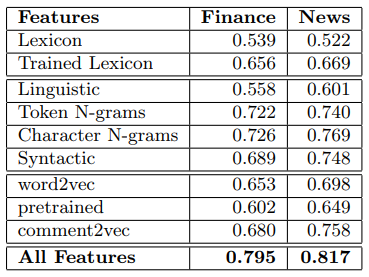
\includegraphics[height=0.3\textheight]{figuras/tabela-modelo-trab2.png}
  \caption{Tabela de resultados para os atributos utilizados do modelo de predição com \textit{F1-Score} \cite{nobata2016abusive}.}
  \label{fig:tb2resultmodel}
\end{figure}


\section{Comentários Ofensivos na Web Brasileira}\label{sec:trabrel-br}
No trabalho \cite{Pelle2017} é apresentado um conjunto de dados com comentários ofensivos (e não ofensivos) coletados na web brasileira. Juntamente com os dados, é apresentado resultados de algoritmos de classificação que servem como base para demais trabalhos futuros.

Os dados foram extraídos de um site brasileiro de notícias, dentre eles foram selecionado 1.250 comentários aleatoriamente. Seguindo o padrão adotado para a classificação dos dados, cada comentário foi anotado por três pessoas com o objetivo de dizer se o comentário é ofensivo ou não.

Foram criadas duas base de dados. A primeira, chamada de {\it OffComBR-2}, possui todos os 1.250 registros (419 classificados como ofensivo) e a classificação atribuída a cada comentário foi determinada por pelo menos duas pessoas. Já a segunda base de dados, {\it OffComBR-3}, possui 1.033 registros (202 ofensivos) e cada comentário foi classificado pelas três pessoas.

Para a classificação dos textos foram criados algumas conjuntos para testes, utilizando métodos PLN, totalizando 24 amostras, 12 para cada base de dados, como podem ser visualizadas na Figura \ref{fig:pelle-statistic}, na qual é possível ver o nome de cada conjunto e o número de características. Segue abaixo os métodos utilizados para formação dos conjuntos:

\begin{itemize}
    \item Redução do Texto: Nesse método, é criado conjuntos de dados com o texto original ({\it original}) e outros com o texto em caixa baixa ({\it lower}).
    \item Tokenização: O texto é dividido em {\it tokens}, onde cada {\it token} é formado por {\it n-grams} e cada {\it unigram} (${1G}$), {\it unigram} e {\it bigram} (${1G+2G}$) e {\it unigram}, {\it bigram} e {\it trigram} (${1G+2G+3G}$) são combinados. Cada {\it token} representa como uma nova característica no conjunto a ser classificado.
    \item Ganho de informação: É selecionado somente características e tem correlação positiva com a classe a ser predita (${FS}$).
\end{itemize}

\begin{figure}[ht]
  \centering
  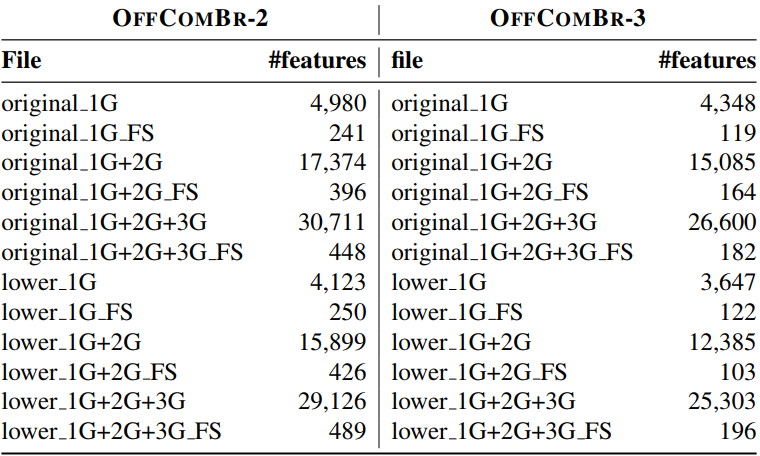
\includegraphics[height=0.3\textheight]{figuras/stats-datasets-offcombr.png}
  \caption{Estatística dos conjuntos de dados \cite{Pelle2017}.}
  \label{fig:pelle-statistic}
\end{figure}

Os algoritmos usado para realizar a classificação do texto foram SVM ({\it Support Vector Machine}) e NB ({\it Naive Bayes}). Como mostra na Figura \ref{fig:pelle-results}, SVM teve um melhor resultado em ambas as base de dados. A base de dados {\it OffComBR-3} teve um melhor resultado, pois a pré-classificação de texto ofensivo está mais definida, onde o texto ofensivo foi classificado pelas três pessoas, ao contrário da {\it OffComBR-2}.

\begin{figure}[ht]
  \centering
  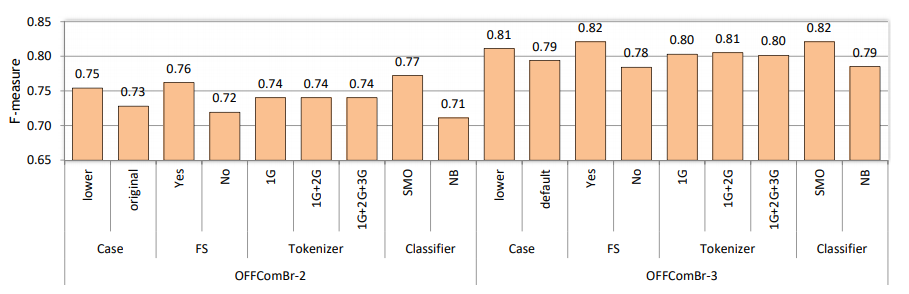
\includegraphics[height=0.2\textheight]{figuras/results-datasets-offcombr.png}
  \caption{Resultados da Classificação dos textos para cada conjunto de características \cite{Pelle2017}.}
  \label{fig:pelle-results}
\end{figure}

\section{Extração de meta-atributos}\label{sec:trabrel-2}

O trabalho \cite{canutoestudo} apresenta um estudo sobre extração de meta-atributos para classificação de textos. Meta-atributos são, em geral, manualmente projetados e extraídos de outros atributos na qual o conjunto de treinamento já é rotulado, e capturam relações fundamentais entre o par \textit{(documento, classe)} ou a tripla \textit{(documento, classe, algoritmo)}. 

Os meta-atributos são capturados usando a  vizinhança de um certo documento de teste a ser classificado utilizando o algoritmo de KNN para identificar os $K$ vizinhos próximos. O trabalho apresenta um estudo comparativo entre utilizar somente meta-atributos, somente os atributos originais da classificação de textos e combinar meta-atributos com os atributos originais.

% meta-atributos
Os meta-atributos baseados em KNN ($M = {mf}$) propostos  contém os vetores de meta-atributos expressos como a concatenação dos sub-vetores descritos a seguir. Cada vetor de atributos $mf$ é definido para um exemplo $xf \in X$ e categoria $cj \in C$ para $j = 1, 2, ... , m$. Segue abaixo os três meta-atributos propostos no artigo:

\begin{itemize}
    \item ${\vec{v}_\vec{x_f}}^{cnt} = [n_j]$:  consiste em um vetor de uma dimensão (tamanho 1) dado pela contagem dos $n_j$ vizinhos (entre os $k$ vizinhos) de $\vec{x_f}$ que são exemplos de treino associados à determinada categoria $c_j$.
    \item ${\vec{v}_\vec{x_f}}^{ncnt} = [\frac{n_j}{n_{max}}]$: consistem em um vetor unidimensional dado pelo número $n_j$ de vizinhos (entre os $k$ vizinhos) de $\vec{x_f}$. O valor de $n_{max}$ corresponde ao número de exemplos associados à classe com o maior número de exemplos dentre os vizinhos mais próximos.
    \item ${\vec{v}_\vec{x_f}}^{qrt} = [\cos{(\vec{x}_{ej}, \vec{x_f})}]$: um vetor de dimensão 5 produzido ao considerar cinco pontos que caracterizam a distribuição de distâncias de $\vec{x_f}$ para seus $j$ vizinhos de dada categoria. As distâncias entre dois vetores $\vec{a}$ e $\vec{b}$ são computadas por similaridade do cosseno, denotada como $\cos{(\vec{a}, \vec{b})}$. Entre todos os pontos de distância entre $\vec{x_f}$ e seus $j$ vizinhos de dada categoria, os cinco pontos selecionados $\cos{(\vec{x}_{1j}, \vec{x_f})}, \cos{(\vec{x}_{2j}, \vec{x_f})}, ... , \cos{(\vec{x}_{5j}, \vec{x_f})}$ correspondem, respectivamente, à menor distância, à
maior distância, à distância média, o quartil inferior (valor que delimita os 25\% dos menores pontos) e o quartil superior (valor que delimita os 25\% dos maiores pontos).
\end{itemize}

Os meta-atributos descritos acima tem uma dimensão de $7$ por categoria. Esse pequeno conjunto de meta-atributos é capaz de capturar informação do conjunto rotulado de três diferentes formas (conforme descrito nos itens acima). A primeira simplesmente conta o número de exemplos rotulados de cada categoria entre os $k$ mais similares exemplos rotulados. A segunda divide o número de vizinhos em cada classe pelo número de vizinhos da classe com maior número de vizinhos, com objetivo de capturar a relação entre a classe escolhida pelo KNN (a classe com maior número de vizinhos) e as outras classes. A última informação fornecida com os meta-atributos propostos é baseada em uma análise das distâncias e distribuição das classes observada na vizinhança do exemplo. Os pontos que caracterizam essas informações são: a menor distância, a maior distância, a mediana, o quartil inferior e o quartil superior.

Os experimentos realizados são em cinco coleções de textos amplamente utilizadas na literatura de classificação automática de texto:

\begin{enumerate}
    \item \textit{4 Universities (4UNI)}. Essa coleção contém páginas da Web coletadas de departamentos de Ciência da Computação de quatro universidades. Existe ao todo 8.277 páginas Web, classificadas em 7 categorias;
    \item \textit{Reuters (REUT)}. Coleção de textos classificados, com artigos de notícias coletados e anotados. Foram considerados 8.184 artigos, classificados em 8 categorias;
    \item \textit{ACM-DL (ACM)}. Um subconjunto da Biblioteca Digital da ACM, com 24.897 documentos contendo artigos relacionados à ciência da computação. Foi considerado apenas o primeiro nível de taxonomia adotado pela ACM, onde cada documento é associado a uma das 11 classes;
    \item \textit{20 Newsgroups (20NG)}. É uma coleção composta de aproximadamente 18.805 documentos de grupo de notícias particionados (aproximadamente) de forma uniforme entre 20 diferentes categorias;
    \item \textit{Spambase (SPAM)}. Uma coleção com diferentes tipos de e-mail. Há um total de 4.601 e-mails classificados como spam ou não-spam;
\end{enumerate}

Os meta-atributos foram avaliados usando duas medidas padrão de classificação de textos: \textit{micro averaged} F1 (MicroF1) que mede a eficácia da classificação sobre todas as decisões, e a \textit{macro averaged} F1 (MacroF1) que mede a eficácia da classificação para cada classe individualmente e obtém a média. Todos os experimentos foram feitos utilizando validação cruzada com 5 partições.

Para a execução dos experimentos e realização da predição dos textos, foi utilizado o algoritmo \textit{SVM}. O tamanho da vizinhança para o algoritmo \textit{KNN} responsável pela geração dos meta-atributos foi definido como sendo \textit{K = 30} (valor tradicionalmente adotado em classificação de texto) para todos os experimentos.
